\documentclass{article}
\usepackage{minted}
\usepackage{graphicx}
\usemintedstyle{colorful}
\usepackage{changepage}
\usepackage[margin = 1.5cm]{geometry}
\usepackage{booktabs}

%\graphicspath{ {C:\Users\Jurek\Documents\Uni\Master\Semester 2\Computational Macro\ar-7-team-computational-tools} }

\title{Assignment 2}
\begin{document}
\maketitle

\definecolor{bg}{rgb}{0.95, 0.95, 0.95}
This document describes our process to code the conditional and unconditional likelihood functions for the AR(7) process based on the starter code provided in the assignment.
Furthermore, it outlines our approach to estimate the AR(7) paramteres for the \texttt{INDPRO} variable from the FRED-MD dataset and our forecast.

\tableofcontents

\section{Conditional Likelihood}
\subsection{Theoretical Outline}
The AR(7) Model is defined as:
\begin{equation}
y_t = c + \phi_1 y_{t-1} + \phi_2 y_{t-2} + \phi_3 y_{t-3} + \phi_4 y_{t-4} + \phi_5 y_{t-5} + \phi_6 y_{t-6} + \phi_7 y_{t-7} + u_t
\end{equation}
where $u_t \sim N(0, \sigma^2)$.

We can then define the conditional likelihood function as:
\begin{equation}
L(y,\phi) = f(y_1, y_2, y_3, y_4, y_5, y_6, y_7;\phi)\prod_{t=8}^Tf(y_t|y_{t-1},..., y_{t-7};\phi)
\end{equation}
The conditional log-likelihood function is:
\begin{equation}
\ell (y; \phi) = \log( f(y_1,..., y_7;\phi))+\sum_{t=8}^T \log (f(y_t|y_{t-1},..., y_{t-7};\phi))
\end{equation}

We regard the first 7 observation or their joint distribution as a determenistic quantity and thus:

\begin{equation}
\ell (y; \phi) \propto \sum_{t=8}^T \log(f(y_t|y_{t-1},..., y_{t-7};\phi))
\end{equation}
Also, since the error terms are normally distributed with mean 0 and varieance $\sigma^2$, we can determine the conditional distribution of $y_t$ as:
\begin{equation}
y_t|y_{t-1},y_{t-2}, ..., y_{t-7} \sim N(c + \phi_1y_{t-1} + ... + \phi_7 y_{t-7}, \sigma^2)
\end{equation}
Therefore, to implement the conditional log-likelihood function we can code it as the sum of normally distributed variables.

\begin{equation}
\ell_C (y; \phi) \propto \sum_{t=8}^T \log \left( \frac{1}{\sigma \sqrt{2\pi}} \exp \left\{-\frac{(y_t - (c+ \phi_1y_{t-1} + ... + \phi_7 y_{t-7} ))^2}{2\sigma^2} \right\} \right)
\end{equation}
\subsection{Implementation in Python}

\begin{minted}[bgcolor=bg]{python}
from scipy.stats import norm
from scipy.stats import multivariate_normal
import numpy as np

def lagged_matrix(Y, max_lag=7):
    n = len(Y)
    lagged_matrix = np.full((n, max_lag), np.nan)    
    # Fill each column with the appropriately lagged data
    for lag in range(1, max_lag + 1):
        lagged_matrix[lag:, lag - 1] = Y[:-lag]
    return lagged_matrix


def cond_loglikelihood_ar7(params, y):
    c = params[0] 
    phi = params[1:8]
    sigma2 = params[8]
    mu, Sigma, stationary = unconditional_ar_mean_variance(c, phi, sigma2)
    ## We could check that at phis the process is stationary and return -Inf if it is not
    if not(stationary):
        return -np.inf
    ## The distribution of 
    # y_t|y_{t-1}, ..., y_{t-7} ~ N(c+\phi_{1}*y_{t-1}+...+\phi_{7}y_{t-7}, sigma2)
    ## Create lagged matrix
    X = lagged_matrix(y, 7)
    yf = y[7:]
    Xf = X[7:,:]
    loglik = np.sum(norm.logpdf(yf, loc=(c + Xf@phi), scale=np.sqrt(sigma2)))
    return loglik
\end{minted}

\section{Unconditional Likelihood}
\subsection{Theoretical Outline}
The unconditional likelihood function starts from a similar approach.
However, instead of regarding the first 7 observations as determenistic it regards them as multivariate normally distributed with mean $\mu$ and covariance $\Sigma$.
\begin{equation}
\ell_U (y; \phi) = \log( f(y_1,..., y_7;\phi, \mu, \Sigma))+\sum_{t=8}^T \log (f(y_t|y_{t-1},..., y_{t-7};\phi))
\end{equation}
The second term on the right hand side is the conditional log-likelihood, the first term is the multivariate normal distribution of the first seven observations.

As described in the assignment the parameters of the multivariate normal distribution can be obtained through:
\begin{equation}
\mu = (I - A)^{-1}b
\end{equation}
to compute the mean and the Lyapunov equation
\begin{equation}
\Sigma = A \Sigma A^T + Q
\end{equation}
to compute the covariance matrix of the autoregressive process.

\subsection{Implementation in Python}
First, the matrix $A$ is constructed, which is a square matrix where the first row is made up of $\phi_1, \phi_2, ..., \phi_p$ of the autoregressive process of order $p$ and the other rows are in reduced row echelon form.

For this the command \mintinline{python}{np.zeros((p,p))} is used, which creates an array of dimension $p \times p$ filled with zeros. 
Next, we replace the first row with $\phi_1, \phi_2, ..., \phi_p$ by subsetting $A$ with the command \mintinline{python}{A[0, :] = phis}.
Next, to fill the remaining rows except the last row with leading ones the comman np.eye is used.

Thus for given $p$ and vector $\phi$, this code creates the matrix $A$ and then calculates the mean and the covariance. 
The code also checks whether the AR(7) process is stationary with respect to the given parameters.
\begin{adjustwidth}{-2cm}{-2cm}
\begin{minted}[bgcolor=bg]{python}
def unconditional_ar_mean_variance(c, phis, sigma2):
    ## The length of phis is p
    p = len(phis)
    A = np.zeros((p, p))
    A[0, :] = phis
    A[1:, 0:(p-1)] = np.eye(p-1)
    ## Check for stationarity
    eigA = np.linalg.eig(A)
    if all(np.abs(eigA.eigenvalues)<1):
        stationary = True
    else:
        stationary = False
    # Create the vector b
    b = np.zeros((p, 1))
    b[0, 0] = c
    
    # Compute the mean using matrix algebra
    I = np.eye(p)
    mu = np.linalg.inv(I - A) @ b
    
    # Solve the discrete Lyapunov equation
    Q = np.zeros((p, p))
    Q[0, 0] = sigma2
    #Sigma = np.linalg.solve(I - np.kron(A, A), Q.flatten()).reshape(7, 7)
    Sigma = scipy.linalg.solve_discrete_lyapunov(A, Q)
    
    return mu.ravel(), Sigma, stationary
\end{minted}
\end{adjustwidth}

This function is used to build the unconditional likelihood function:

\begin{minted}[bgcolor=bg]{python}
def uncond_loglikelihood_ar7(params, y):
    ## The unconditional loglikelihood
    ## is the unconditional "plus" the density of the
    ## first p (7 in our case) observations
    cloglik = cond_loglikelihood_ar7(params, y)

    ## Calculate initial
    # y_1, ..., y_7 ~ N(mu, sigma_y)
    c = params[0] 
    phi = params[1:8]
    sigma2 = params[8]
    mu, Sigma, stationary = unconditional_ar_mean_variance(c, phi, sigma2)
    if not(stationary):
        return -np.inf
    mvn = multivariate_normal(mean=mu, cov=Sigma, allow_singular=True)
    uloglik = cloglik + mvn.logpdf(y[0:7])
    return uloglik
\end{minted}
\section{Maximum Likelihood Estimation for \texttt{INDPRO}}
As in assignment 1, we import the FRED-MD dataset using \texttt{pandas}.
Since we are only interested in the \texttt{INDPRO} variable, we select it and transform it using log differences:
\begin{minted}[bgcolor=bg]{python}
import pandas as pd
import numpy as np
#Read Data
df = df = pd.read_csv('~/Downloads/current.csv')
#Select INDPRO
INDPRO = df['INDPRO']
#Drop first Row
INDPRO = INDPRO.drop(index=0)
#transform INDPRO using log differences
INDPRO = np.log(INDPRO).diff()

#implement Starter Code from the assignment
## Lagged Matrix Function
def lagged_matrix(Y, max_lag=7):
    n = len(Y)
    lagged_matrix = np.full((n, max_lag), np.nan)    
    # Fill each column with the appropriately lagged data
    for lag in range(1, max_lag + 1):
        lagged_matrix[lag:, lag - 1] = Y[:-lag]
    return lagged_matrix

## Mean- Variance - Stationarity Function
def unconditional_ar_mean_variance(c, phis, sigma2):
    ## The length of phis is p
    p = len(phis)
    A = np.zeros((p, p))
    A[0, :] = phis
    A[1:, 0:(p-1)] = np.eye(p-1)
    ## Check for stationarity
    eigA = np.linalg.eig(A)
    if all(np.abs(eigA.eigenvalues)<1):
        stationary = True
    else:
        stationary = False
    # Create the vector b
    b = np.zeros((p, 1))
    b[0, 0] = c
    
    # Compute the mean using matrix algebra
    I = np.eye(p)
    mu = np.linalg.inv(I - A) @ b
    
    # Solve the discrete Lyapunov equation
    Q = np.zeros((p, p))
    Q[0, 0] = sigma2
    #Sigma = np.linalg.solve(I - np.kron(A, A), Q.flatten()).reshape(7, 7)
    Sigma = scipy.linalg.solve_discrete_lyapunov(A, Q)
    
    return mu.ravel(), Sigma, stationary

## Conditional Likelihood
def cond_loglikelihood_ar7(params, y):
    c = params[0] 
    phi = params[1:8]
    sigma2 = params[8]
    mu, Sigma, stationary = unconditional_ar_mean_variance(c, phi, sigma2)
    ## We could check that at phis the process is stationary and return -Inf if it is not
    if not(stationary):
        return -np.inf
    ## The distribution of 
    # y_t|y_{t-1}, ..., y_{t-7} ~ N(c+\phi_{1}*y_{t-1}+...+\phi_{7}y_{t-7}, sigma2)
    ## Create lagged matrix
    X = lagged_matrix(y, 7)
    yf = y[7:]
    Xf = X[7:,:]
    loglik = np.sum(norm.logpdf(yf, loc=(c + Xf@phi), scale=np.sqrt(sigma2)))
    return loglik

## Unconditional Likelihood
def uncond_loglikelihood_ar7(params, y):
    ## The unconditional loglikelihood
    ## is the unconditional "plus" the density of the
    ## first p (7 in our case) observations
    cloglik = cond_loglikelihood_ar7(params, y)

    ## Calculate initial
    # y_1, ..., y_7 ~ N(mu, sigma_y)
    c = params[0] 
    phi = params[1:8]
    sigma2 = params[8]
    mu, Sigma, stationary = unconditional_ar_mean_variance(c, phi, sigma2)
    if not(stationary):
        return -np.inf
    mvn = multivariate_normal(mean=mu, cov=Sigma, allow_singular=True)
    uloglik = cloglik + mvn.logpdf(y[0:7])
    return uloglik
    
# Using INDPRO as the target variable.
## Computing OLS
X = lagged_matrix(INDPRO, 7)
yf = INDPRO[7:]
Xf = np.hstack((np.ones((len(INDPRO)-7,1)), X[7:,:]))
beta = np.linalg.solve(Xf.T@Xf, Xf.T@yf)
sigma2_hat = np.mean((yf - Xf@beta)**2)
params= np.hstack((beta, sigma2_hat))
print("The parameters of the OLS model are", params)

# to maximize likelihood a function of the negative likelihood is defined to be minimized
params = np.array([
    0.0012, ## c
    0.0291, 0.07, 0.059, 0.04, 0.04, 0.02, 0.06, ## phi
    0.008 ## sigma2    
    ])

def cobj(params, y): 
    return - cond_loglikelihood_ar7(params,y)

#Same Procedure for unconditional likelihood
params= np.hstack((beta, sigma2_hat))
\end{minted}
As the next step we construct the matrix containing \texttt{INDPRO} and its lagged values .

\subsection{Results: Conditional Likelihood}
\subsubsection{Unconstrained Maximization}
We estimate four different models for the conditional likelihood:
\begin{enumerate}
\item \texttt{Model 1}: We use the OLS coefficients as the initial guess and minimize the conditional likelihood function using the 'L-BFGS-B' method.
\item \texttt{Model 2}: We use the OLS coefficients as the initial guess and minimize the conditional likelihood function using the 'Neler-Mead' method.
\item \texttt{Model 3}: We supply a different initial guess and minimize the conditional likelihood function using the 'L-BFGS-B' method.
\item \texttt{Model 4}: We supply a different initial guess and minimize the conditional likelihood function using the  'Neler-Mead' method.
\end{enumerate}

\begin{minted}[bgcolor=bg]{python}

# Now we estimate multiple models:
## OLS model
modOLS = np.hstack((beta, sigma2_hat))
## Conditional Likelihood
## 1. Using the OLS parameters as the initial guess
### L-BFGS-B
mod1 = scipy.optimize.minimize(fun = cobj, x0 =  modOLS, args = INDPRO, method='L-BFGS-B').x
### Nelder-Mead
mod2 = scipy.optimize.minimize(fun = cobj, x0 =  modOLS, args = INDPRO, method='Nelder-Mead').x
## 2. Using a slightly different initial guess
Initial_Guess = np.array([
    0.0012, ## c
    0.0291, 0.07, 0.059, 0.04, 0.04, 0.02, 0.06, ## phi
    0.009 ## sigma2 
])
### L-BFGS-B
mod3 = scipy.optimize.minimize(fun = cobj, x0 =  Initial_Guess, args = INDPRO, method='L-BFGS-B').x
### Nelder-Mead
mod4 = scipy.optimize.minimize(fun = cobj, x0 =  Initial_Guess, args = INDPRO, method='Nelder-Mead').x

# Compiling models to print to LateX table
def as_latex_table(rows, rownames, colnames, caption):
    df = np.array(rows)
    df = pd.DataFrame(df)
    df = df.T
    df.insert(0, colnames[1], rownames)
    df.columns = column_names
    tabular = df.to_latex(index=False,
                           caption=caption)
    return tabular

column_names = ("Coefficients", "OLS", "Model 1", "Model 2", "Model 3", "Model 4")
rownames = ["$c$", "$\\phi_1$", "$\\phi_2$", "$\\phi_3$", "$\\phi_4$", 
            "$\\phi_5$", "$\\phi_6$", "$\\phi_7$", "$\\sigma^2$"]
caption="Results of the unconstrained maximization of the conditional likelihood"
print(as_latex_table([modOLS, mod1, mod2, mod3, mod4], 
	rownames=rownames, colnames=column_names, caption=caption))
\end{minted}

The results are displayed in Table 1.
The results show that if the initial guess are the OLS coefficients, the conditional MLE correctly finds identical coefficients. However, when we supply a different initial guess, the minimization procedure using 'L-BFGS-B' returns simply the same initial guess while using the 'Neler-Mead' method changes the estimated coefficients quite dramatically.\\

\begin{table}[h]
\centering
\caption{Results of the unconstrained maximization of the conditional likelihood}
\begin{tabular}{lrrrrr}
\toprule
Coefficients & OLS & Model 1 & Model 2 & Model 3 & Model 4 \\
\midrule
$c$ & 0.001263 & 0.001263 & 0.001263 & 0.001200 & 0.000874 \\
$\phi_1$ & 0.291263 & 0.291263 & 0.291263 & 0.029100 & 0.056374 \\
$\phi_2$ & -0.074517 & -0.074517 & -0.074517 & 0.070000 & 0.017666 \\
$\phi_3$ & 0.046809 & 0.046809 & 0.046809 & 0.059000 & 0.060468 \\
$\phi_4$ & 0.047565 & 0.047565 & 0.047565 & 0.040000 & 0.009790 \\
$\phi_5$ & -0.024910 & -0.024910 & -0.024910 & 0.040000 & 0.058602 \\
$\phi_6$ & 0.061501 & 0.061501 & 0.061501 & 0.020000 & 0.038055 \\
$\phi_7$ & 0.020106 & 0.020106 & 0.020106 & 0.060000 & 0.114138 \\
$\sigma^2$ & 0.000089 & 0.000089 & 0.000089 & 0.009000 & 0.000095 \\
\bottomrule
\end{tabular}
\end{table}

\subsubsection{Constrained Maximization}
As discussed in the previous section, the unconstrained likelihood maximization faced several issues.
The reason for this, as error messages made clear, is that using unbounded optimization, leads to negative values in $\sigma^2$ which created errors in:
\mint{python}|scale=np.sqrt(sigma2)|
Using the constraint $\sigma^2 \geq 0$
\mint{python}|bounds_sigma = tuple((0,np.inf) for _ in range(1))|
similarly created error messages, since $\sigma$ enters into the denominaor in the PDF of the normal distribution.
Thus, we decided to use the constraint: $\sigma^2 > 0$, i.e. $\sigma^2$ must be strictly larger than zero, which yielded estimated parameters close to the OLS estimate even when using very different initial guesses.
We reestimated Models 1-4 using constrained maximization:
\begin{minted}[bgcolor=bg]{python}
## We then reestimate these models unsing constrained maximization:
bounds_constant = tuple((-np.inf, np.inf) for _ in range(1))
bounds_phi = tuple((-1, 1) for _ in range(7))
bounds_sigma = tuple((0.000001,np.inf) for _ in range(1))
bounds = bounds_constant + bounds_phi + bounds_sigma

## Conditional Likelihood
## 1. Using the OLS parameters as the initial guess
### L-BFGS-B
mod1 = scipy.optimize.minimize(fun = cobj, x0 =  modOLS, args = INDPRO, method='L-BFGS-B', bounds=bounds).x
### Nelder-Mead
mod2 = scipy.optimize.minimize(fun = cobj, x0 =  modOLS, args = INDPRO, method='Nelder-Mead', bounds=bounds).x
## 2. Using a slightly different initial guess
Initial_Guess = np.array([
    0.0012, ## c
    0.0291, 0.07, 0.059, 0.04, 0.04, 0.02, 0.06, ## phi
    0.009 ## sigma2 
])
### L-BFGS-B
mod3 = scipy.optimize.minimize(fun = cobj, x0 =  Initial_Guess, args = INDPRO, method='L-BFGS-B', bounds=bounds).x
### Nelder-Mead
mod4 = scipy.optimize.minimize(fun = cobj, x0 =  Initial_Guess, args = INDPRO, method='Nelder-Mead', bounds=bounds).x
\end{minted}

\begin{table}[h]
\centering
\caption{Results of the constrained maximization of the conditional likelihood}
\begin{tabular}{lrrrrr}
\toprule
Coefficients & OLS & Model 1 & Model 2 & Model 3 & Model 4 \\
\midrule
$c$ & 0.001263 & 0.001263 & 0.001263 & 0.001283 & 0.000874 \\
$\phi_1$ & 0.291263 & 0.291263 & 0.291263 & 0.283561 & 0.056374 \\
$\phi_2$ & -0.074517 & -0.074517 & -0.074517 & -0.018719 & 0.017666 \\
$\phi_3$ & 0.046809 & 0.046809 & 0.046809 & 0.003397 & 0.060468 \\
$\phi_4$ & 0.047565 & 0.047565 & 0.047565 & 0.031652 & 0.009790 \\
$\phi_5$ & -0.024910 & -0.024910 & -0.024910 & -0.010921 & 0.058602 \\
$\phi_6$ & 0.061501 & 0.061501 & 0.061501 & 0.029010 & 0.038055 \\
$\phi_7$ & 0.020106 & 0.020106 & 0.020106 & 0.039583 & 0.114138 \\
$\sigma^2$ & 0.000089 & 0.000089 & 0.000089 & 0.000089 & 0.000095 \\
\bottomrule
\end{tabular}
\end{table}

As the table shows, even when choosing an initial guess different from the OLS parameters the bounded optimization yields largely accurate estimates when using the 'L-BFGS-B' method.

\subsection{Results: Unconditional Likelihood}
\subsubsection{Unconstrained Maximization}
We estimate the following models for the unconditional likelihood function:
\begin{itemize}
\item \texttt{Model 5}: We use the OLS coefficients as the initial guess and minimize the unconditional likelihood function using the 'L-BFGS-B' method.
\item \texttt{Model 6}: We use the OLS coefficients as the initial guess and minimize the unconditional likelihood function using the 'Neler-Mead' method.
\end{itemize}

\begin{minted}[bgcolor=bg]{python}
## Unbounded Unconditional Likelihood
## 1. Using the OLS parameters as the initial guess
### L-BFGS-B
mod5 = scipy.optimize.minimize(fun = uobj, x0 =  modOLS, args = INDPRO, method='L-BFGS-B').x
### Nelder-Mead
mod6 = scipy.optimize.minimize(fun = uobj, x0 =  modOLS, args = INDPRO, method='Nelder-Mead').x
## 2. Using a slightly different initial guess
Initial_Guess = np.array([
    0.0012, ## c
    0.00291, 0.007, 0.0509, 0.0024, 0.0409, 0.012, 0.0601, ## phi
    0.009 ## sigma2 
])
### L-BFGS-B
#mod7 = scipy.optimize.minimize(fun = uobj, x0 =  Initial_Guess, args = INDPRO, method='L-BFGS-B').x
### Nelder-Mead
#mod8 = scipy.optimize.minimize(fun = uobj, x0 =  Initial_Guess, args = INDPRO, method='Nelder-Mead').x
\end{minted}
The results are displayed in Table 2:
\begin{minted}[bgcolor=bg]{python}
umods = np.array([modOLS, mod5, mod6])
umodsDF = pd.DataFrame(umods)
umodsDF = umodsDF.T
rownames = ["$c$", "$\phi_1$", "$\phi_2$", "$\phi_3$", "$\phi_4$", 
            "$\phi_5$", "$\phi_6$", "$\phi_7$", "$\sigma^2$"]
umodsDF.insert(0, "Coefficients", rownames)
column_names = ("Coefficients", "OLS", "Model 5", "Model 6")
umodsDF.columns = column_names
print(umodsDF.to_latex())
\end{minted}

\begin{table}[h]
\centering
\caption{Results of the unconstrained maximization of the unconditional likelihood}
\begin{tabular}{lrrr}
\toprule
Coefficients & OLS & Model 5 & Model 6 \\
\midrule
$c$ & 0.001263 & 0.001263 & 0.001277 \\
$\phi_1$ & 0.291263 & 0.291263 & 0.309304 \\
$\phi_2$ & -0.074517 & -0.074517 & -0.076766 \\
$\phi_3$ & 0.046809 & 0.046809 & 0.040008 \\
$\phi_4$ & 0.047565 & 0.047565 & 0.038904 \\
$\phi_5$ & -0.024910 & -0.024910 & -0.031723 \\
$\phi_6$ & 0.061501 & 0.061501 & 0.056227 \\
$\phi_7$ & 0.020106 & 0.020106 & 0.020665 \\
$\sigma^2$ & 0.000089 & 0.000091 & 0.000091 \\
\bottomrule
\end{tabular}
\end{table}
\subsubsection{Constrained Maximization}
We introduce two further models analagous to the earlier section to see whether using a different initial guess yields reliable results.
\begin{itemize}
\item \texttt{Model 7}: Bounded optimization using 'L-BFGS-B'
\item \texttt{Model 8}: Bounded optimization using 'Nelder-Mead'
\end{itemize}

\begin{table}[h]
\centering
\caption{Results of the constrained maximization of the unconditional likelihood}
\begin{tabular}{lrrrrr}
\toprule
Coefficients & OLS & Model 5 & Model 6 & Model 7 & Model 8 \\
\midrule
$c$ & 0.001263 & 0.001263 & 0.001277 & 0.001142 & 0.001462 \\
$\phi_1$ & 0.291263 & 0.291263 & 0.309304 & 0.287896 & 0.009534 \\
$\phi_2$ & -0.074517 & -0.074517 & -0.076766 & 0.007889 & -0.014135 \\
$\phi_3$ & 0.046809 & 0.046809 & 0.040008 & 0.030199 & 0.079556 \\
$\phi_4$ & 0.047565 & 0.047565 & 0.038904 & 0.024074 & -0.005964 \\
$\phi_5$ & -0.024910 & -0.024910 & -0.031723 & 0.001736 & 0.050275 \\
$\phi_6$ & 0.061501 & 0.061501 & 0.056227 & 0.025235 & 0.043152 \\
$\phi_7$ & 0.020106 & 0.020106 & 0.020665 & 0.049086 & 0.034731 \\
$\sigma^2$ & 0.000089 & 0.000091 & 0.000091 & 0.000092 & 0.000100 \\
\bottomrule
\end{tabular}
\end{table}

\section{Forecast}
We use the estimated parameters to generate forecasts for \texttt{INDPRO} eight periods ahead.
For this purpose we define a function, which takes the forecast horizon and the estimated model parameters as inputs, using the aforementioned eight periods and the OLS coefficients as defaults.

\begin{minted}[bgcolor=bg]{python}
### Forecasting:
def forecastAR(h=8, model = mods[0]): # defaults: h is the forecasting horizon, mods[0] the OLS model
    forecastArray = np.empty(h) # Empty array to store forecasts
    lastrow = np.array(INDPRO.tail(7)) #use last 7 rows of INDPRO for the first forecast
    lastrow = np.flip(lastrow) # invert array to align with order of estimated parameters in the model
    for i in range(1, h+1):
        forecast = model[0] + model[1:8] @ lastrow + np.random.normal(scale=np.sqrt(model[8]))# mods[0] uses the OLS estimates
        lastrow = np.insert(lastrow, 0, forecast)
        lastrow = np.delete(lastrow, -1)
        forecastArray[i-1] = forecast

    return forecastArray
\end{minted}
\subsection{Forecast: Conditional Likelihood}
Again we display the results in a Table.
\begin{minted}[bgcolor=bg]{python}
rownames = ("$y_{t+1}$", "$y_{t+2}$", "$y_{t+3}$", "$y_{t+4}$",
            "$y_{t+5}$","$y_{t+6}$", "$y_{t+7}$", "$y_{t+8}$")
results = {'Forecasts': rownames,'OLS': forecastAR(), 'Model 1': forecastAR(model = mods[1]),
           'Model 2': forecastAR(model = mods[2]),'Model 3': forecastAR(model = mods[3]),
           'Model 4': forecastAR(model = mods[4])}
results = pd.DataFrame(results)

caption="Forecasts using the estimated coefficients from OLS and the bounded conditional likelihood maximization."
print(results.to_latex(index=False, caption=caption))
\end{minted}

\begin{table}[h]
\centering
\caption{Forecasts using the estimated coefficients from OLS and the bounded conditional likelihood maximization.}
\begin{tabular}{lrrrrr}
\toprule
Forecasts & OLS & Model 1 & Model 2 & Model 3 & Model 4 \\
\midrule
$y_{t+1}$ & -0.001868 & 0.005603 & 0.001309 & -0.001886 & -0.005620 \\
$y_{t+2}$ & -0.004988 & -0.011386 & 0.003612 & 0.000642 & -0.007806 \\
$y_{t+3}$ & -0.003126 & -0.009734 & 0.003625 & -0.001772 & -0.006855 \\
$y_{t+4}$ & 0.005572 & 0.000821 & -0.011357 & 0.007225 & -0.006454 \\
$y_{t+5}$ & 0.018263 & -0.000091 & 0.013110 & 0.010745 & -0.013280 \\
$y_{t+6}$ & 0.007414 & 0.012544 & 0.015779 & 0.012925 & -0.002697 \\
$y_{t+7}$ & 0.010241 & -0.003814 & 0.009928 & -0.001046 & 0.005218 \\
$y_{t+8}$ & -0.001302 & 0.010320 & 0.008232 & -0.002915 & 0.006240 \\
\bottomrule
\end{tabular}
\end{table}

\subsection{Forecast: Unconditional Likelihood}
\begin{minted}[bgcolor=bg]{python}
rownames = ("$y_{t+1}$", "$y_{t+2}$", "$y_{t+3}$", "$y_{t+4}$",
            "$y_{t+5}$","$y_{t+6}$", "$y_{t+7}$", "$y_{t+8}$")
results = {'Forecasts': rownames,'OLS': forecastAR(), 'Model 5': forecastAR(model = mods[5]),
           'Model 6': forecastAR(model = mods[6]),'Model 7': forecastAR(model = mods[7]),
           'Model 8': forecastAR(model = mods[8])}
results = pd.DataFrame(results)

caption="Forecasts using the estimated coefficients from OLS and the bounded unconditional likelihood maximization."
print(results.to_latex(index=False, caption=caption))
\end{minted}
\begin{table}[h]
\centering
\caption{Forecasts using the estimated coefficients from OLS and the bounded unconditional likelihood maximization.}
\begin{tabular}{lrrrrr}
\toprule
Forecasts & OLS & Model 5 & Model 6 & Model 7 & Model 8 \\
\midrule
$y_{t+1}$ & -0.002498 & -0.006758 & 0.009115 & -0.001652 & -0.006767 \\
$y_{t+2}$ & -0.004464 & 0.001639 & 0.007614 & -0.000249 & 0.003534 \\
$y_{t+3}$ & -0.012308 & -0.011037 & -0.020483 & 0.003442 & 0.016761 \\
$y_{t+4}$ & -0.024551 & -0.006179 & -0.014886 & 0.006549 & 0.019912 \\
$y_{t+5}$ & -0.008911 & -0.010317 & -0.005740 & 0.011542 & -0.005094 \\
$y_{t+6}$ & -0.010678 & 0.001352 & 0.008654 & 0.020144 & -0.002298 \\
$y_{t+7}$ & -0.005979 & 0.004190 & 0.004085 & 0.016980 & 0.003778 \\
$y_{t+8}$ & 0.016936 & 0.006097 & 0.020236 & -0.014125 & -0.000141 \\
\bottomrule
\end{tabular}
\end{table}

\subsection{Comparing Forecasts}
Since the models which use OLS as the initial guess yield forecasts equal to the OLS forecasts, we focus here on the models using bounded optimization and the 'L-BFGS-B' method.
We compute their respective deviation from the OLS forecasts and the sum of the squared deviations.
As table 7 shows, the deviations are quite small, but since the forecast contains a random term these will vary.
\begin{table}[h]
\centering
\caption{Forecasts using OLS, Model 3 (Bounded Conditional Likelihood, Different Initial Guess), Model 7(Bounded Unconditional Likelihood, Different Initial Guess)}
\begin{tabular}{llllrr}
\toprule
Forecasts & OLS & Model 3 & Model 7 & OLS - Model 3 & OLS - Model 7 \\
\midrule
$y_{t+1}$ & -0.007050041 & -0.005532853 & 0.005141836 & -0.001517188 & -0.012191877 \\
$y_{t+2}$ & 0.001975987 & -0.003519636 & 0.002374953 & 0.005495623 & -0.000398965 \\
$y_{t+3}$ & -0.013918260 & -0.014313323 & 0.009323091 & 0.000395062 & -0.023241351 \\
$y_{t+4}$ & -0.001553839 & 0.010026787 & 0.000272816 & -0.011580627 & -0.001826656 \\
$y_{t+5}$ & 0.006570045 & -0.011069952 & 0.008189258 & 0.017639997 & -0.001619213 \\
$y_{t+6}$ & 0.007944712 & -0.008128802 & 0.001483508 & 0.016073514 & 0.006461204 \\
$y_{t+7}$ & 0.006855851 & -0.001665351 & 0.005689299 & 0.008521202 & 0.001166552 \\
$y_{t+8}$ & -0.017166112 & 0.006106558 & -0.002798542 & -0.023272670 & -0.014367570 \\
$\sum \Delta^2$ &   &   &   & 0.001350526 & 0.000944455 \\
\bottomrule
\end{tabular}
\end{table}
\subsection{Evaluating Forecasts}
Here we choose a grahpical display. 
The idea is to choose a certain date, for example 01/01/2000 and train a model on all observations up to this date.
Then, we estimate the next $h$ perionds and compare them to the actual values.
This code produces such a plot displaying the actual values, the OLS forecasts and forecasts generated by models 3 and 7, that is bounded maximum likelihood estimation using `L-BFGS-B'.
\begin{minted}[bgcolor=bg]{python}
# Task 4: Comparing Forecasts by plotting them
# plotting forecasts:
# Using the data up to 2000 as training data and the rest of the data as testing data
# Creating a new dataframe containgin all the data up to a certain date, say for example 01/01/2020 and forecasted data from there onwards to compare
# actual to forecasted data.
df = df.drop(index=0)
df['sasdate'] = pd.to_datetime(df['sasdate'])
date = "01/01/2000"
lasttrain = df.index[df['sasdate']== date].to_list() 
train = INDPRO[:lasttrain[0]]
test = INDPRO[lasttrain[0]-1:]

#First, OLS Model:
X = lagged_matrix(train, 7)
yf = train[7:]
Xf = np.hstack((np.ones((len(train)-7,1)), X[7:,:]))
beta = np.linalg.solve(Xf.T@Xf, Xf.T@yf)
sigma2_hat = np.mean((yf - Xf@beta)**2)
params= np.hstack((beta, sigma2_hat))
modOLS = params

#Second, conditional likelihood:
modCon = scipy.optimize.minimize(fun = cobj, x0 =  Initial_Guess, args = train, method='L-BFGS-B', bounds=bounds).x

#Third, unconditional likelihood:
modUCon = scipy.optimize.minimize(fun = uobj, x0 =  Initial_Guess, args = train, method='L-BFGS-B', bounds=bounds).x

mods = np.array([modOLS, modCon, modUCon])
def forecastAR(h=8, model = mods[0], data=train): # defaults: h is the forecasting horizon, mods[0] the OLS model
    forecastArray = np.empty(h) # Empty array to store forecasts
    lastrow = np.array(data.tail(7)) #use last 7 rows of test data for the first forecast
    lastrow = np.flip(lastrow) # invert array to align with order of estimated parameters in the model
    for i in range(1, h+1):
        forecast = model[0] + model[1:8] @ lastrow + np.random.normal(scale=np.sqrt(model[8])) # mods[0] uses the OLS estimates
        lastrow = np.insert(lastrow, 0, forecast)
        lastrow = np.delete(lastrow, -1)
        forecastArray[i-1] = forecast

    return forecastArray


h = 8 # forecast for h periods
forecast={'INDPRO': test[:h], 
          'Forecast OLS': forecastAR(h=h), 
          'Forecast Conditional': forecastAR(h=h, model = mods[1]),
          'Forecast Unconditional': forecastAR(h=h, model = mods[2])}

forecast = pd.DataFrame(forecast)

plotdata = {'INDPRO': train, 
            'Forecast OLS': train, 
            'Forecast Conditional': train,
            'Forecast Unconditional': train}

plotdata = pd.DataFrame(plotdata)
plotdata =  [plotdata, forecast]
plotdata = pd.concat(plotdata)
plotdata.insert(0, "sasdate",df.iloc[1:len(plotdata)+1,0])
plotdata = plotdata.tail(2*h) # seletct the h forecasted observations and the h previous observations for plotting.
print(plotdata)

plt.plot(plotdata['sasdate'], plotdata['Forecast OLS'], color = "blue")
plt.plot(plotdata['sasdate'], plotdata['Forecast Conditional'], color = "green")
plt.plot(plotdata['sasdate'], plotdata['Forecast Unconditional'], color = "red")
plt.plot(plotdata['sasdate'], plotdata['INDPRO'],color="black")
plt.legend(['Forecast OLS', 'Forecast Conditional', 'Forecast Unconditional', 'INDPRO'])
plt.show()
\end{minted}

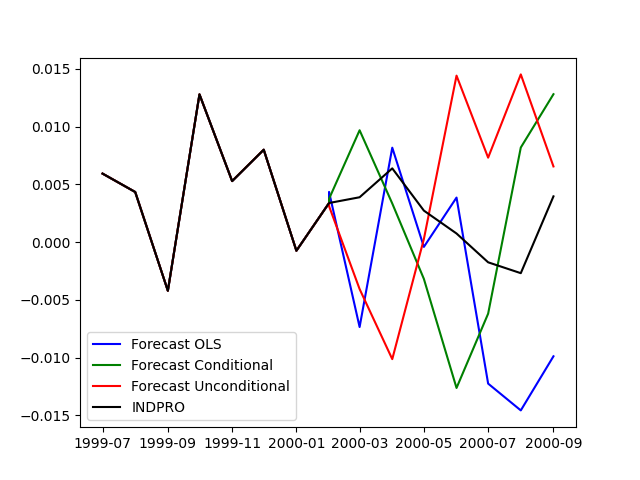
\includegraphics{Figure.png}

\end{document}